\chapter{Bestimmung des totalen Stoßwirkungsquerschnitts}

\subsection{Physikalische Grundlagen}

\paragraph{Compton-Streuung}

Die in diesem Versuch eingesetzte $\gamma$-Strahlung stammt aus dem Zerfall von $^{137}$Cs und besitzt eine Energie von etwa $661{,}7\,\mathrm{keV}$. 
In diesem Energiebereich dominiert die Compton-Streuung die Wechselwirkung der Photonen mit Materie. 
Dabei wird ein Photon an einem quasi freien Elektron gestreut und überträgt einen Teil seiner Energie auf dieses Elektron.

Die Energie des gestreuten Photons hängt vom Streuwinkel $\theta$ ab und wird durch die Compton-Beziehung beschrieben \cite{Wermes}:

\begin{align}
    E'_\gamma = \frac{E_\gamma}
    {1+\frac{E_\gamma}{m_e c^2}(1-\cos\theta)}
    \label{eq:compton}
\end{align}

Hierbei bezeichnet $m_e$ die Elektronenmasse und $c$ die Lichtgeschwindigkeit.

\paragraph{Abschwächung der Strahlung}

Da die Bindungsenergien der Elektronen im Aluminium im Vergleich zur Photonenergie klein sind, können die Elektronen näherungsweise als frei betrachtet werden. 
Die Intensitätsabnahme der $\gamma$-Strahlung beim Durchgang durch Materie lässt sich mit dem Lambert-Beer-Gesetz \cite{compton_uzh} beschreiben:

\begin{align}
    I(d)=I_0 e^{-\mu d}
    \label{eq:beer}
\end{align}

Dabei ist $I_0$ die Anfangsintensität, $d$ die Materialdicke und $\mu$ der lineare Schwächungskoeffizient.

Der totale Wirkungsquerschnitt $\sigma$ \cite{Knoll}\cite{Leo} ergibt sich über die Elektronendichte des Materials zu

\begin{align}
    \sigma = \frac{\mu}{n_e},
\end{align}

wobei die Elektronendichte \cite{Knoll}\cite{Leo} durch

\begin{align}
    n_e = \frac{Z \rho N_A}{M}
\end{align}

gegeben ist. 
Hierbei stehen $Z$ für die Ordnungszahl, $\rho$ für die Dichte, $M$ für die molare Masse und $N_A$ für die Avogadro-Konstante.

Im betrachteten Energiebereich spielt die Paarbildung keine Rolle, da hierfür mindestens $1{,}022\,\mathrm{MeV}$ erforderlich wären. 
Der Photoeffekt liefert in Aluminium lediglich einen kleinen Beitrag zur Gesamtabschwächung.

\section{Versuchsdurchführung}

Zur Bestimmung des totalen Stoßwirkungsquerschnitts wurde der Versuchsaufbau so eingestellt, dass ausschließlich der Primärstrahl detektiert wird (Konfiguration 1). 
Hierzu wurden Aluminiumabsorber unterschiedlicher Dicke in den Strahlengang eingebracht.

Für jede Dicke erfolgte eine Messung über einen Zeitraum von $600\,\mathrm{s}$, um vergleichbare statistische Unsicherheiten zu erhalten. 
Durch die Wechselwirkung der $\gamma$-Strahlung mit dem Material nimmt die Intensität des transmittierten Strahls mit wachsender Absorberdicke ab.

\paragraph{Totzeitkorrektur}

Der verwendete Detektor besitzt eine endliche Totzeit $\tau$. 
Während dieser Zeit können keine weiteren Ereignisse registriert werden. 
Insbesondere bei hohen Zählraten führt dies zu einer systematischen Unterschätzung der tatsächlichen Intensität.

Die korrigierte Zählrate ergibt sich aus

\begin{align}
    R_\mathrm{true}
    =
    \frac{R_\mathrm{meas}}
    {1-R_\mathrm{meas}\tau}.
\end{align}

\paragraph{Einfluss der Rotation}

Zusätzlich wurde untersucht, wie sich eine Verdrehung des Targets auf die effektive Materialdicke auswirkt. 
Wird der Absorber um einen Winkel $\alpha$ gedreht, verlängert sich der effektive Weg der Photonen im Material gemäß

\begin{align}
    d_\mathrm{eff}=\frac{d}{\cos\alpha}.
\end{align}

Für eine Rotation um $45^\circ$ ergibt sich somit eine effektive Dickenzunahme um den Faktor $\sqrt{2}$.

\section{Auswertung}

Die aufgenommenen Spektren für verschiedene Aluminiumdicken sind in Abb.~\ref{plot:csue} dargestellt. 
Im Bereich kleiner Kanalnummern ist das Compton-Kontinuum sichtbar, während der Photopeak des $^{137}$Cs-Zerfalls bei etwa Kanal $6500$ deutlich hervortritt.

\begin{figure}[htbp]
    \centering
    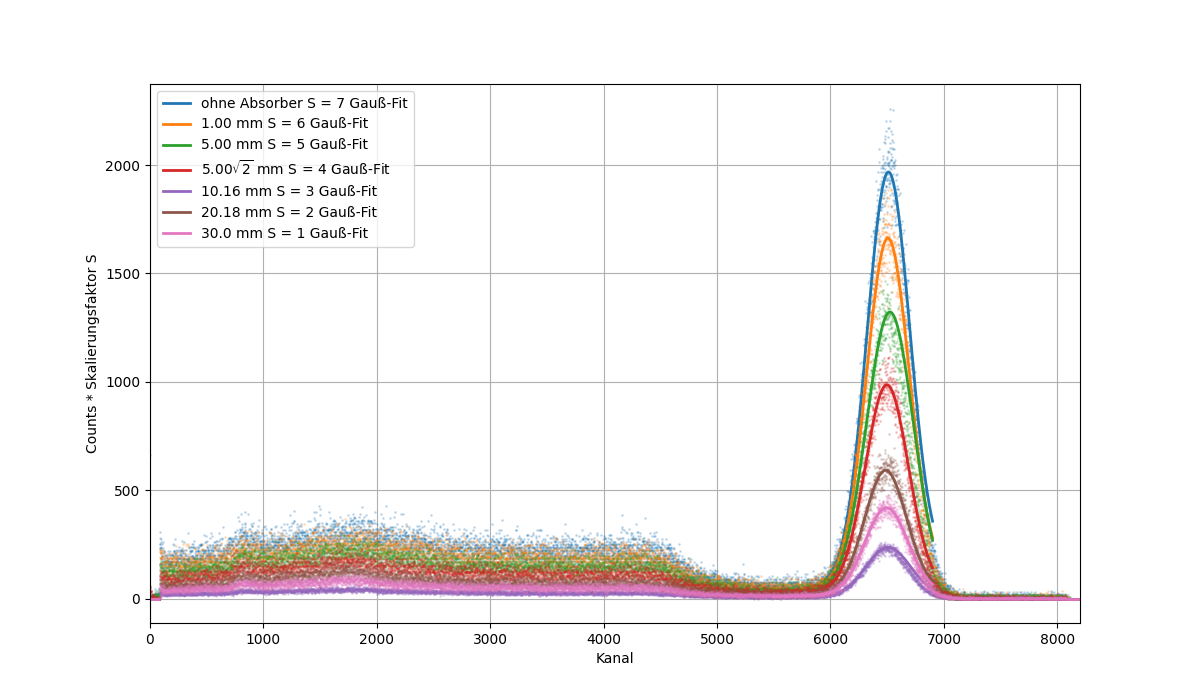
\includegraphics[width=0.75\textwidth]{figs/Cäsium überlappen.png}
    \caption{Vergleich der aufgenommenen Spektren für verschiedene Absorberdicken. 
    Zur besseren Sichtbarkeit wurden die Spektren individuell skaliert. 
    Die Anpassung der Photopeaks erfolgte mit einer Gaußfunktion gemäß Gl.~\ref{eq:gauss}.}
    \label{plot:csue}
\end{figure}

Die Lage der Peaks bleibt innerhalb der Unsicherheiten konstant, während die Peakamplitude mit zunehmender Materialdicke abnimmt. 
Dies entspricht der erwarteten Abschwächung der $\gamma$-Strahlung.

Zur Beschreibung der Photopeaks wurde eine Gaußfunktion verwendet:

\begin{align}
    G(x)=
    \frac{A}{\sqrt{2\pi}\sigma}
    \exp\left[
    -\frac{(x-\mu)^2}{2\sigma^2}
    \right]
    \label{eq:gauss}
\end{align}

Die erhaltenen Fitparameter sind in Tab.~\ref{tab:gauss_parameter_cssp} zusammengefasst.

\begin{table}[htbp]
\centering
\caption{Fitparameter der Gaußanpassung für unterschiedliche Absorberdicken.}
\begin{tabular}{ccccc}
\hline
Dicke/mm  & $A$ & $\mu$ & $\sigma$ & $\chi^2_\mathrm{red}$ \\
\hline
0,00 & $690,30 \pm 8,57$ & $6517,33 \pm 5,55$ & $195,05 \pm 2,85$ & 0,875 \\
1,00 & $678,24 \pm 7,89$ & $6510,88 \pm 5,27$ & $193,52 \pm 2,76$ & 0,914 \\
5,00 & $645,48 \pm 8,73$ & $6523,20 \pm 6,25$ & $204,90 \pm 3,21$ & 0,843 \\
7,07 & $598,95 \pm 6,41$ & $6497,93 \pm 5,05$ & $191,35 \pm 2,77$ & 0,851 \\
10,16 & $576,79 \pm 7,26$ & $6511,28 \pm 5,93$ & $200,51 \pm 3,16$ & 0,795 \\
20,18 & $478,80 \pm 5,20$ & $6488,94 \pm 5,21$ & $188,58 \pm 2,97$ & 0,810 \\
30,00 & $509,47 \pm 5,85$ & $6496,79 \pm 5,49$ & $192,84 \pm 3,05$ & 0,824 \\
\hline
\end{tabular}
\label{tab:gauss_parameter_cssp}
\end{table}

Die reduzierten $\chi^2$-Werte liegen in allen Fällen nahe bei Eins, was auf eine gute Beschreibung der Messdaten durch die Gaußfunktion hinweist.

Aus den Peakflächen wurde anschließend die Abschwächung der Intensität bestimmt. 
Da die gemessenen Counts proportional zur Intensität sind, folgt aus Gl.~\ref{eq:beer}

\begin{align}
    \ln\left(\frac{I_0}{I(d)}\right)
    =
    \mu d.
\end{align}

Die entsprechenden Werte sind in Tab.~\ref{tab:totw} dargestellt.

\begin{table}[htbp]
\centering
\caption{Logarithmische Intensitätsabschwächung in Abhängigkeit der Absorberdicke.}
\begin{tabular}{cc}
\hline
Dicke/mm & $\ln(I_0/I)$ \\
\hline
$1,00 \pm 0,02$ & $-0,00670 \pm 0,00611$ \\
$5,00 \pm 0,02$ & $0,04438 \pm 0,00618$ \\
$7,07 \pm 0,08$ & $0,07692 \pm 0,00626$ \\
$10,16 \pm 0,02$ & $0,12430 \pm 0,00631$ \\
$20,18 \pm 0,02$ & $0,27400 \pm 0,00661$ \\
$30,00 \pm 0,02$ & $0,22340 \pm 0,00651$ \\
\hline
\end{tabular}
\label{tab:totw}
\end{table}

Der Messpunkt bei $30\,\mathrm{mm}$ wurde bei der linearen Regression nicht berücksichtigt, da dieser deutlich vom erwarteten Verlauf abweicht. 
Eine mögliche Ursache ist die begrenzte geometrische Ausdehnung des Absorbers, wodurch sich die effektive Detektionswahrscheinlichkeit verändert.

\begin{figure}[htbp]
    \centering
    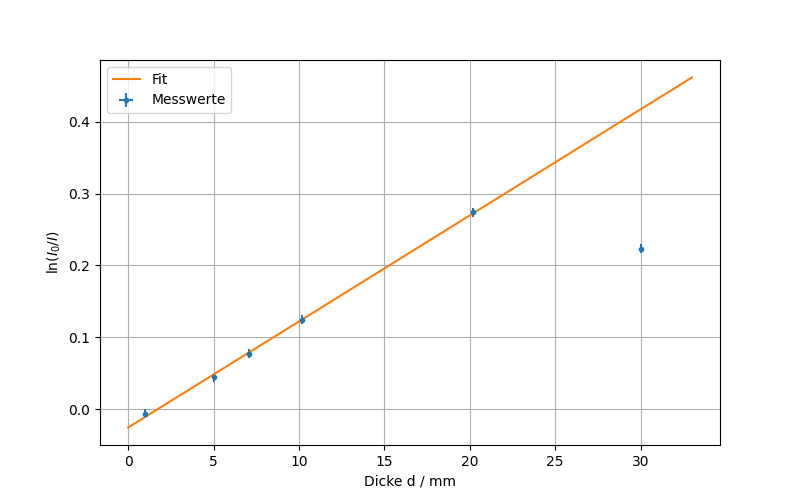
\includegraphics[width=0.75\textwidth]{figs/totalerwirkungsquerschnitt_nicht_durch0.png}
    \caption{Lineare Darstellung der logarithmischen Intensitätsabschwächung in Abhängigkeit der Absorberdicke.}
    \label{plot:totw}
\end{figure}

Aus der Steigung der Ausgleichsgeraden ergibt sich der lineare Schwächungskoeffizient zu

\begin{align}
    \mu = (0,0148 \pm 0,0004)\,\mathrm{mm^{-1}}.
\end{align}

Unter Verwendung der Materialparameter von Aluminium ergibt sich daraus ein totaler Wirkungsquerschnitt von

\begin{align}
    \sigma_\mathrm{tot}
    =
    (188,6 \pm 5,7)\,\mathrm{mb}.
\end{align}

Der Literaturwert beträgt etwa $257\,\mathrm{mb}$ \cite{sigmalit}. 
Der experimentell bestimmte Wert liegt damit deutlich unterhalb des Literaturwertes.

Mögliche Ursachen für diese Abweichung sind systematische Effekte des Messaufbaus sowie Vereinfachungen in der Auswertung. 
Insbesondere wurde angenommen, dass die Abschwächung ausschließlich durch Compton-Streuung verursacht wird. 
Zusätzliche Beiträge durch den Photoeffekt oder Streuprozesse innerhalb des Aufbaus können das Ergebnis beeinflussen.

Darüber hinaus können Oxidschichten auf den Aluminiumtargets die effektive Elektronendichte verändern. 
Ebenso ist es möglich, dass gestreute Photonen trotz Richtungsänderung weiterhin im Detektor registriert werden und dadurch die gemessene Transmission erhöhen.

Trotz der systematischen Abweichung liefert die Messung insgesamt die erwartete Größenordnung des totalen Stoßwirkungsquerschnitts von $\gamma$-Strahlung in Aluminium.
